\section{Experiments}
\label{sec:induced_experiments}
In this section, we first describe our dataset, followed by our experimental setup; comparative baselines, evaluation metrics, and implementation details. We then present results across several experiments to evaluate the performance of our model on merging semantically diverse induced-relations.

\subsection{Dataset}
We first evaluate our approach on multiple communities catering to different topics from a popular online Community Question Answer (CQA) platform, \emph{StackExchange\footnote{https://stackexchange.com/}}. The platform divides the communities into five different categories, i.e. Technology ($\mathbf{T}$), Culture/Recreation ($\mathbf{C}$), Life/Arts ($\mathbf{L}$), Science ($\mathbf{S}$) and Professional ($\mathbf{P}$).
For our analysis, we collect data from the ten largest communities from each of the five categories until March 2019, resulting in a total of 50 StackExchange communities.
The list of 50 StackExchange communities per category are;
\begin{itemize}
\item Technology: AskUbuntu, Server Fault, Unix, TEX, Electronics, Gis, Apple, Wordpress, Drupal, DBA
\item Culture/Recreation: English, Travel, RPG, Judaism, Puzzling, Bicycles, German, Christianity, BoardGames, History
\item Life/Arts: Scifi, DIY, Academia, Graphic Design, Money, Photo, WorldBuilding, Movies, Music, Law
\item Science: Stat, Physics, MathOverflow, CS, Chemistry, Biology, Philosophy, CS Theory, Economics, Astronomy

\item Professional/Business: Workplace, Aviation, Writers, Open source, Freelancing, CS Educators, Quant, PM, Parenting
\end{itemize}
In StackExchange, each questioner can mark a candidate answer as an "accepted" answer. We only consider questions with an accepted answer. Table \ref{tab:stats} shows the final dataset statistics.


\begin{table*}[h]
 \centering
 \begin{subtable}{\linewidth}
 \setlength{\tabcolsep}{3pt}
   \begin{tabular}{l | c c c | c c c | c c c }
  \toprule
  &  \multicolumn{3}{c}{{Technology}} &
  \multicolumn{3}{c}{{Culture/Recreation}} &
  \multicolumn{3}{c}{{Life/Arts}} \\
  & ServerFault & AskUbuntu & Unix & English & Games & Travel & SciFi & Home & Academia \\ \midrule
$\vert Q \vert$ & 61,873 & 41,192 & 9,207 & 30,616 & 12,946 & 6,782 & 14,974 & 8,022 & 6,442  \\
$\vert  \mathcal{A} \vert$ & 181,974 & 119,248 & 33,980 & 110,235 & 45,243 & 20,766 & 49,651& 23,956 & 23,837 \\
$ \vert U \vert$ & 140,676 & 200,208 & 84,026 & 74,592 & 14,038 & 23,304 & 33,754 & 30,698 & 19,088 \\
$ \mu (\vert  \mathcal{A}_q \vert) $ & 2.94 & 2.89 & 3.69 & 3.6 & 3.49 & 3.06 & 3.31 & 2.99 & 3.7 \\
   \bottomrule
 \end{tabular}%
\end{subtable}\vspace{8mm}

\begin{subtable}{\linewidth}
\centering
 \begin{tabular}{l | c c c | c c c}
\toprule
&
\multicolumn{3}{c}{{Science}} &
\multicolumn{3}{c}{{Professional/Business}}\\
& Physics & Maths & Statistics & Workplace & Aviation & Writing \\ \midrule
$\vert Q \vert$ &  23,932 & 18,464 & 13,773 & 8,118 & 4,663 & 2,932 \\
$\vert  \mathcal{A} \vert$ & 65,800 & 53,772 & 36,022 & 33,220 & 14,137 & 12,009 \\
$ \vert U \vert$ & 52,505 & 28,181 & 54,581& 19,713 & 7,519 & 6,918 \\
$ \mu (\vert  \mathcal{A}_q \vert) $ & 2.75 & 2.91 & 2.62 & 4.09 & 3.03 & 4.10 \\
 \bottomrule
\end{tabular}
\end{subtable}
 \caption{ \label{tab:stats}Dataset statistics for the top three Stack Exchange communities from five different categories. $\vert Q \vert$: number of questions; $\vert  \mathcal{A} \vert$: number of answers; $ \vert U \vert $: number of users; $ \mu (\vert  \mathcal{A}_q \vert) $: mean number of answers per question. Professional/Business communities have slightly more answers per question on average than others. Technology communities are the largest in terms of number of question out of the five categories.}
\end{table*}

For each $(q, a)$ tuple, we compute the following basic features:\\
\emph{Activity features :} View count of the question, number of comments for both question and answer, the difference between posting time of question and answer, arrival rank of answer (we assign rank 1 to the first posted answer) \cite{TianZL13}. \\
\emph{Text features :} Paragraph and word count of question and answer, presence of code snippet in question and answer (useful for programming based forums), word count in the question title.\\
\emph{User features :} Word count in user profile's Aboutme section for both users; one who is posting the question and the other posting the answer.

Time-dependent features like upvotes/downvotes of the answer and user features like reputation or badges used in earlier studies on StackExchange \cite{BurelMA16} are problematic for two reasons. First, we only know the aggregate values, not how these values change with time. Second, since these values typically increase over time, it is unclear if an accepted answer received the votes \emph{prior} to or \emph{after} an answer was accepted. Thus, we do not use such time-dependent features for our model and the baselines in our experiments.

\textbf{Reddit\footnote{https://www.reddit.com/}} is another popular CQA platform with subreddits similar to StackExchange communities. In particular, we focus on Ask* subreddits as they are primarily used to seek help from a community of experts and non-experts. In particular, we crawled data from /r/askscience (science forum), /r/AskHistorians (history forum), and /r/AskDocs (medical forum) until October 2017. We performed basic preprocessing and removed posts or comments with single word/URLs or missing author/title information. We also removed infrequent users who posted less than two comments.
Reddit has a hierarchical comment structure. For this paper, we treat first-level comments as potential answers to the question. Users in these subreddits can get verified by providing anonymized verification documents including certification numbers, contact information, etc. to the moderators. We denote these verified users as experts. We treat an expert's comment as equivalent to an accepted answer and only consider posts which have an expert answer for our experiments. We discard posts with multiple experts' comment as it is hard to objectively choose a winner.

\begin{table}[h]
\centering
\begin{tabular}{l  r r r r}
 \toprule
 Dataset & $\vert \mathcal{Q} \vert$ & $\vert \mathcal{A} \vert$ & $\vert \mathcal{U} \vert$ & $ \mu (\vert  \mathcal{A}_q \vert) $ \\  \midrule
 AskDocs & 11189 & 29207& 4530 & 2.61               \\
 AskHistorians & 15425 & 45586 & 11761 & 2.96                     \\
 AskScience & 37990 & 121278 & 32117 & 3.19                 \\
  \bottomrule
\end{tabular}
  \caption{Dataset statistics for the Ask* Reddit communities. $\vert Q \vert$: number of questions; $\vert  \mathcal{A} \vert$: number of answers; $ \vert U \vert $: number of users; $ \mu (\vert  \mathcal{A}_q \vert) $: mean number of answers per question.}
\end{table}

We employ 12 basic features for the Reddit dataset: \\
\emph{Activity features :} ArrivalRank of the answer, number of subsequent comments on the answer, number of other answers to the question, Upvotes and downvotes for both, question and answer.\\
\emph{Text features :} Word count of the question and answer

We employ post-vote features here as \cite{Gilbert:2013} showed that there is widespread under-provision of voting on Reddit, partially due to long comment threads. It can act as a weak signal for answer quality. Unlike the StackExchange, Reddit voting is not biased by publicly visible acceptance of answers to a question. Thus, votes ideally represent the independent judgment of the crowd.


\subsection{Experimental Setup}

\noindent
\textbf{Baselines} We compare against state-of-the-art feature-based baselines for answer selection and competing aggregation approaches to fuse diverse relational views of the dataset~\cite{DualGCN, relationalGCN}.

\noindent
\textit{Random Forest (RF)} \cite{BurelMA16, TianZL13} model trains on the feature set mentioned earlier for each dataset. This model is shown to be the most effective feature-based model for Answer Selection.

\noindent
\textit{Feed-Forward network (FF)} \cite{JendersKN16} is used as a deep learning baseline to learn non-linear transformations of the feature vectors for each $(q, a)$ tuple. This model is equivalent to our Reflexive GCN model in isolation.

\noindent
\textit{Dual GCN (DGCN)} \cite{DualGCN} trains a separate GCN for each view. In addition to the supervised loss computed using training labels, they introduce a regularizer to minimize mean squared error (MSE) between vertex representations of two views, thus aligning the learned latent spaces.
Formally,
For instance,
\begin{equation}
 \mathcal L_{reg}(Z_c, Z_{ts}) = \lVert \mathbf{Z}_c^K - \mathbf{Z}_{ts}^K \lVert
\end{equation}
computes the MSE loss between Contrastive and TrueSkill Similarity GCN.
\citet{DualGCN} proposed the model for two GCN representations and we extend it to four GCN with each GCN representing our relational view.
The Contrastive view is seen to exhibit the best performance in isolation. Thus, the DualGCN loss can be given by:

\begin{equation}
  \mathcal L  = \mathcal L_0 +  \lambda{(t)} \left( \sum_{S_i \in \mathbf{S}, S_i \neq c} \lVert \mathbf{Z}_c^K - \mathbf{Z}_i^K \lVert \right)
\end{equation}
where $\mathcal L_0$ represents the supervised loss and $\mathbf{Z}_c^K$ is the vertex representations of the Contrastive GCN.
The regularizer loss is similar to our intra-relation aggregation approach but assumes label and feature sharing across \emph{all} the views.

\noindent
\textit{Relational GCN (RGCN)} \cite{relationalGCN} combines the output representations of previous layer of each view to compute an aggregated input to the current layer, i.e.,
$\mathbf{Z}_i^{k-1}$ of layer $k-1$ of each view is used to compute an aggregated input to layer $k$.
Formally,

\begin{equation}
  \mathbf{Z}_{rgcn}^{k} = \sigma \left( \sum_{S_i \in \mathbf{S}} \mathbf{Z}_i^{k-1}\right)
\end{equation}
where $Z_{rgcn}$ is final output of this model at layer $k$ and $\sigma$ is the activation function.

We also report results for each view individually: Contrastive (C-GCN), Arrival Similarity (AS-GCN), TrueSkill Similarity (TS-GCN), and Reflexive (R-GCN) with our proposed IR-GCN model. We do not compare with other graph structure-based approaches to compute vertex representations \cite{DeepWalk, node2vec, Planetoid, LINE} as GCN is shown to outperform them \cite{gcn}. We also later compare with common aggregation strategies to merge neural representations discussed earlier in ~\cref{sec:aggregation}.

\noindent
\textbf{Evaluation Metric}
We randomly select 20\% of the questions, $\mathbf{T}_q \subset \mathcal{Q}$ to be in the test set. Then, subsequently all $(q,a)$ tuples such that $q \in \mathbf{T}_q$ comprise the set of test tuples or vertices, $\mathbf{T}$ . The rest of the vertices, along with their label information, is used for training the model.
We evaluate our model on two metrics, Accuracy and Mean Reciprocal Rank (MRR). Accuracy metric is widely used in vertex classification literature while MRR is popular for ranking problems like answer selection. Formally,
\begin{align}
Acc = \frac{1}{\vert \mathbf{T} \vert} \sum_{(q,a) \in  \mathbf{T} } \mathbbm{1} \left(  y_{(q,a)} \cdot h_b((q,a)) > 0 \right)
\end{align}
with $\cdot$ as the product and $\mathbbm{1}(.)$ as the indicator function. The product is positive if the accepted label and predicted label match and negative otherwise.
\begin{equation}
MRR = \frac{1}{\vert \mathbf{T}_q \vert} \sum_{q \in \mathbf{T}_q} \frac{1}{\sum_{a' \in \mathcal{A}(q)}  \mathbbm{1} \left(L_{(q,a)} < L_{(q,a')} \right)}
\end{equation}
 where
$L_{(q,a)}$ refers to the position of accepted answer $a$ in the ranked list for question $q$ \cite{Wang:2009}.

 \begin{table*}[!h]
\begin{threeparttable}[!h]
   \robustify\bfseries
   \centering
  \sisetup{
    table-figures-integer = 3,
    table-figures-decimal = 2,
    separate-uncertainty,
    table-figures-uncertainty = 1
  }
   %\setlength{\tabcolsep}{1pt}
   \begin{subtable}{\textwidth}
    %   \centering
   \resizebox{1\textwidth}{!}{
   %\centering
    \begin{tabular}{l|l l| l l | l l}
     \toprule
     \multirow{2}{*}{Method} &
        \multicolumn{2}{c}{{Technology}} &
       \multicolumn{2}{c}{{Culture/Recreation}} &
       \multicolumn{2}{c}{{Life/Arts}} \\
       &{Acc(\%)} & {MRR}&{Acc(\%)} & {MRR}&{Acc(\%)}& {MRR}\\
       \midrule
     {RF~\cite{BurelMA16, TianZL13}} & 66.78$\pm$0.023 & 0.683$\pm$0.043 & 72.5$\pm$0.018 & 0.626$\pm$0.050 & 72.71$\pm$0.049 & 0.628$\pm$0.089\\


     {FF~\cite{JendersKN16}} & 67.31$\pm$0.027 & 0.786$\pm$0.022 & 72.22$\pm$0.020 & 0.782$\pm$0.023\textbf{*} & 73.58$\pm$0.049 & 0.780$\pm$0.034 \\
     {DGCN~\cite{DualGCN}} & 70.70$\pm$0.022 & 0.782$\pm$0.017 & 75.22$\pm$0.017 & 0.771$\pm$0.028 & 76.73$\pm$0.034 &0.784$\pm$0.038 \\
     {RGCN~\cite{relationalGCN}} & 54.40$\pm$0.045 & 0.673$\pm$0.045 & 60.39$\pm$0.016 & 0.645$\pm$0.042 & 59.97$\pm$0.043 & 0.654$\pm$0.054 \\
     \cmidrule(lr){1-1}\cmidrule(lr){2-7}
     {AS-GCN} & 67.76$\pm$0.032 &0.775 $\pm$0.015 & 73.05 $\pm$0.021 & 0.763$\pm$0.025 &73.79 $\pm$0.048 & 0.776$\pm$0.042 \\
     {TS-GCN} & 66.87$\pm$0.032 & 0.779$\pm$0.018 & 72.16$\pm$0.023 & 0.764$\pm$0.023 & 72.02$\pm$0.061 & 0.765$\pm$0.048 \\
     {C-GCN} & 71.64$\pm$0.022\textbf{*} & 0.790$\pm$0.015\textbf{*}& 76.18$\pm$0.017\textbf{*}& 0.781$\pm$0.024 & 77.37$\pm$0.034\textbf{*}& 0.788$\pm$0.040\textbf{*} \\
     {IR-GCN} & \bfseries 73.96$\pm$\bfseries0.023 & \bfseries0.794$\pm$\bfseries0.014 & \bfseries 78.61$\pm$\bfseries0.018 & \bfseries0.790$\pm$\bfseries0.025 & \bfseries79.21$\pm$\bfseries0.032 & \bfseries0.800$\pm$\bfseries0.037 \\
     \bottomrule
   \end{tabular}
   }
   \end{subtable}\vspace{8mm}
   \begin{subtable}{\textwidth}
   \resizebox{0.73\textwidth}{!}{
   \begin{tabular}{l|l l| l l }
    \toprule
    \multirow{2}{*}{Method} &
      \multicolumn{2}{c}{{Science}} &
      \multicolumn{2}{c}{{Professional/Business}}\\
      & {Acc(\%)} & {MRR}&{Acc(\%)} & {MRR}\\
      \midrule
    {RF~\cite{BurelMA16, TianZL13}} & 68.09$\pm$0.024 & 0.692$\pm$0.049 & 74.72$\pm$0.044 & 0.5951$\pm$0.081\\
    {FF~\cite{JendersKN16}} & 67.87$\pm$0.024 & 0.800$\pm$ 0.028 & 74.63$\pm$0.040 & 0.759$\pm$0.049\\
    {DGCN~\cite{DualGCN}} & 71.45$\pm$0.023\textbf{*} & 0.791$\pm$0.035 & 76.86$\pm$0.031 & 0.751$\pm$0.046\\
    {RGCN~\cite{relationalGCN}} & 58.65$\pm$0.054 & 0.682$\pm$0.042 &63.02$\pm$0.038 & 0.657$\pm$0.061\\
    \cmidrule(lr){1-1}\cmidrule(lr){2-5}%\cmidrule(lr){12-21}
    {AS-GCN} & 66.93$\pm$0.045 & 0.788 $\pm$0.028 & 74.99$\pm$0.045 &0.742 $\pm$0.047\\
    {TS-GCN} & 65.90$\pm$0.042 & 0.790$\pm$0.031 & 74.17$\pm$0.046 &0.747$\pm$0.044\\
    {C-GCN} & 70.81$\pm$0.042 & 0.800$\pm$0.032\textbf{*}& 77.57$\pm$0.038\textbf{*} & 0.768$\pm$0.034\textbf{*}\\
    {IR-GCN} & \bfseries74.98$\pm$\bfseries0.021 & \bfseries0.808$\pm$\bfseries0.028 & \bfseries80.17$\pm$\bfseries0.026 & \bfseries0.785$\pm$\bfseries0.032\\
    \bottomrule
  \end{tabular}
  }
  \end{subtable}
   \begin{tablenotes}
       \footnotesize
       \item[*] DGCN stands for DualGCN, RGCN stands for RelationalGCN, and IR-GCN stands for Induced Relational GCN.
   \end{tablenotes}
   \caption{\label{tab:stackacc} Accuracy and MRR values for StackExchange with state-of-the-art baselines. Our model outperforms by at least 4\% in Accuracy and 2.5\% in MRR. Contrastive GCN performs best among individual views. The model with $*$ symbol has the second-best performance among all other models. Our model shows statistical significance at level 0.01 overall second best model on single tail paired t-test.}
   \end{threeparttable}
 \end{table*}


\noindent
\textbf{Implementation Details}
We implemented our model and the baselines in Pytorch. We use ADAM optimizer \cite{ADAM} for training with 50\% dropout to avoid overfitting. We use four hidden layers in each GCN with hidden dimensions 50, 10, 10, 5, respectively, and ReLU activation. The coefficients of $\mathcal{L}_1$ and $\mathcal{L}_2$ regularizers are set to $\gamma_1 = 0.05$ and $\gamma_2 = 0.01$ respectively. For TrueSkill Similarity, we use margin $\delta = 4$ to create links, while for Arrival similarity, we use $\delta = 0.95$.
We implement a mini-batch version of training for large graphs where each batch contains a set of questions and their associated answers.  This mini-batch version is equivalent to training on the whole graph as we have disconnected cliques.


\subsection{Performance Analysis}
Table \ref{tab:stackacc} shows impressive gains over state-of-the-art baselines for all the five categories of StackExchange. We report mean results for each category obtained after 5-fold cross-validation on each of the communities. Our induced-relational GCN model beats best performing baseline by 4-5\% on average in accuracy. The improvement in MRR values is around 2.5-3\% across all categories. Note that MRR is based only on the rank of the accepted answer, while accuracy is based on correct labeling of \emph{both} accepted and non-accepted answers.

\begin{figure}[h]
  \centering
  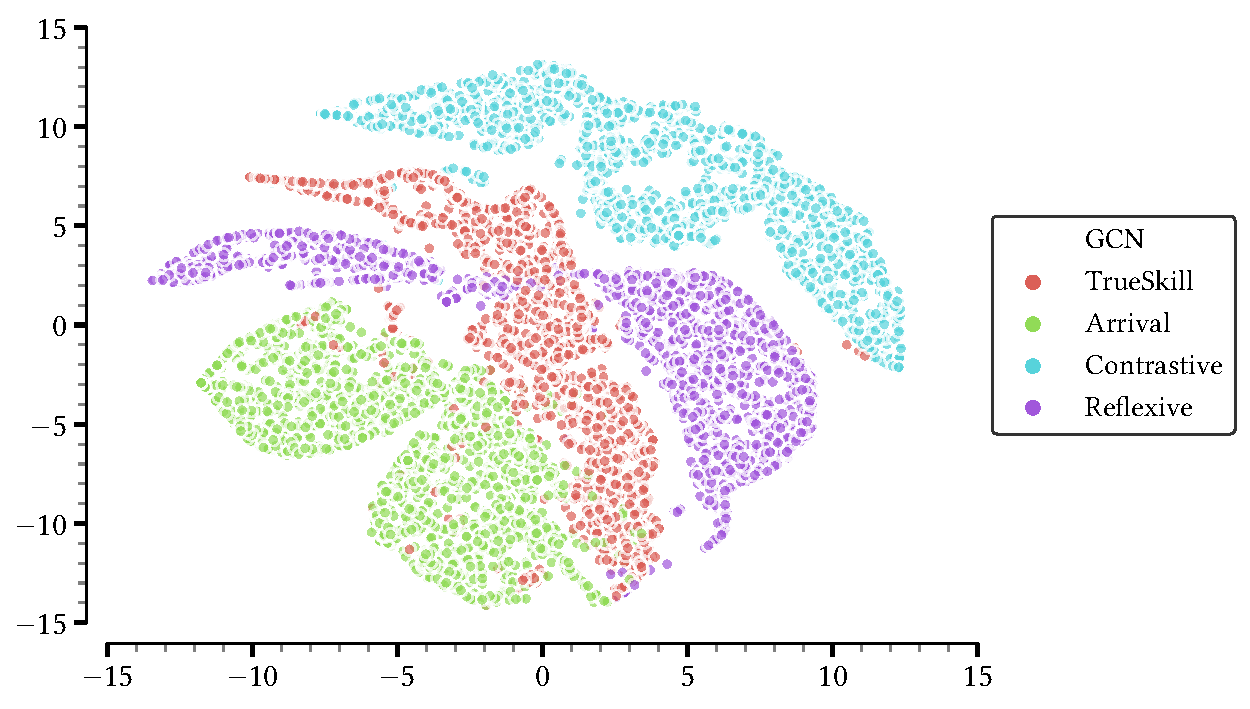
\includegraphics[scale=0.5]{figures/sne_plot.pdf}
  \caption{\label{fig:sne} t-stochastic neighbor embedding (t-SNE) \cite{sne} distributions of the learned vertex representations by our model for Chemistry StackExchange. Each view learns a distinct vertex representation. Best viewed in color.}
\end{figure}

Among individual views, Contrastive GCN performs best on all the communities. It even beats the best performing baseline DualGCN that uses all the relational views. Note that the contrastive view compares between the candidate answers to a question and uses our proposed contrastive modification to the convolution operation. Arrival Similarity follows Contrastive and then Reflexive. The superior performance of the Arrival Similarity view shows that early answers tend to get accepted and vice versa. It indicates that users primarily use CQA forums for quick answers to their queries. Also, recall that Reflexive predicts each vertex's label independent of other answers to the same question. Thus, the competitive performance of the Reflexive strategy indicates that vertex's features itself are well predictive of the label. TrueSkill Similarity performs at par or slightly worse than Reflexive. \Cref{fig:sne} presents t-SNE distributions \cite{sne} of the learned vertex representations ($\mathbf{Z}_i^K$) of our model applied to Chemistry StackExchange from Science category. Note that each view, including two views under Similar Contrast relation, learns a distinct vertex representation. Hence, all views are essential and contribute to our final performance.

Out of the baseline graph ensemble approaches, DualGCN performs significantly better than RelationalGCN by an average of around 26\% for all categories. Recall that in the RelationalGCN model, the convolution output of each view is linearly combined to compute the final output. Linear combination works well for knowledge graphs as each view can be thought of as a feature, and then it accumulates information from each feature. DualGCN is similar to our approach and trains different GCN for each view and later merges their results. However, it enforces similarity in vertex representations learned by each view. This restriction is not suitable for our induced-relationships as they are semantically different (contrastive captures contrast in features vs. similarity enforces label sharing).

\begin{table}[tbh]
  \robustify\bfseries
  \centering
  \sisetup{
    table-figures-integer = 3,
    table-figures-decimal = 2,
    separate-uncertainty,
    table-figures-uncertainty = 1
  }
  \begin{tabular}{l| c c c c c c}
    \toprule
    \multirow{2}{*}{{Method}} &
      \multicolumn{2}{c}{{AskDocs}} &
      \multicolumn{2}{c}{{AskHistorians}} &
      \multicolumn{2}{c}{{AskScience}} \\
      & {Acc (\%)} & {MRR} & {Acc(\%)} & {MRR} & {Acc(\%)} & {MRR} \\
      \midrule
    RF~\cite{BurelMA16, TianZL13} & 59.35 & 0.698 & 65.62 & 0.709 & 65.87 & 0.706  \\
    FF~\cite{JendersKN16} & 62.30 & 0.715 & 67.89 & 0.7302 & 68.99 & 0.713  \\
    DGCN~\cite{DualGCN} & 77.54 & 0.790 & 80.49 & 0.805 & 75.57 & 0.821 \\
    RGCN~\cite{relationalGCN} & 57.98 & 0.667 & 64.56 & 0.684 & 62.42 & 0.642 \\
    \midrule
    AS-GCN & 76.53 & 0.794 & 80.70 & 0.781 & 78.14 & 0.797 \\
    TS-GCN & 84.44 & 0.861 & 90.95 & 0.829 & 87.61 & 0.822 \\
    C-GCN & 67.39 & 0.753 & 70.57 & 0.744 & 71.11 & 0.769 \\
    IR-GCN & \textbf{87.60} &  \textbf{0.896} &  \textbf{93.81} &  \textbf{0.851} &  \textbf{89.11} &  \textbf{0.837} \\
    \bottomrule
  \end{tabular}
  \caption{\label{tab:reddit} Accuracy and MRR values for Ask\* Reddits. Our model significantly outperforms by 16\% in Accuracy and 7\% in MRR. TrueSkill Similarity performs best among individual IR-GCNs.}
\end{table}

Table \ref{tab:reddit} shows performance gains over the state-of-art baselines for the Reddit dataset. All results are reported after 5-fold cross-validation. Our model improves by 16\% on average in accuracy over the baselines for Reddit. The improvement in MRR is at an average increase of 7\% than the baseline higher than for StackExchange.

Among individual views, for Reddit, there is a considerable difference in performance for each view. TrueSkill Similarity performs much better, followed by Arrival Similarity and Contrastive. Reflexive GCN performs the worst for Reddit as it predicts each node's label independent of answers to the same question.

Out of the baseline graph ensemble approaches, DualGCN and RelationalGCN, similar to StackExchange, DualGCN consistently performs better than RelationalGCN by an average of around 3\% for Reddit.

\section{Discussion}
\label{sec:discussion}
In this section, we first evaluate the importance of each relational view for our boosted model. We then compare with approaches proposed to merge neural networks in general in other domains. We then illustrate \emph{discriminative magnification effect} in detail and study the robustness of our model to training label sparsity.  We also extend our proposed approach to include textual features and compare it with a text-based model. Finally, we provide a theoretical analysis of performance gains of our Contrastive GCN model and provide limitations of our approach.

\subsection{Ablation Study on Relation Types}
\begin{table}[h]
 \centering
  \robustify\bfseries
  \begin{tabular}{l | c | c| c| c|c | c}
    \toprule
       {\{ Relation Type\}} &
        {Tech} &
        {Culture} &
        {Life} &
        {Sci}&
        {Business} & {AskDocs}\\
      \midrule
      C & 71.23 &75.90 &78.71&72.99 & 76.85 & 67.39\\
    \{ TS, AS \} & 67.86 &74.15 &75.75&65.80& 76.13 & 84.57 \\
    R & 68.30 & 73.35 & 76.57 & 67.40 & 75.76 & 62.30\\
    \{TS, AS \} + R & 69.28 & 75.50 &76.41 &70.11 &77.90 & 86.34  \\
    C + R & 73.04 & 77.66 & 80.25 &73.72 & 80.04 & 70.02\\
    C + \{ TS, AS \} & 72.81 & 78.04 & 81.41 & 72.19 & 80.15 & 86.99\\
    C + \{ TS, AS \} + R & \bfseries 73.87 & \bfseries 78.74 & \bfseries 81.60&  \bfseries74.68&  \bfseries80.56 & \bfseries 87.60\\
    \bottomrule
  \end{tabular}
  \caption{\label{tab:relation} 5-fold Accuracy (in \%) comparison for different combination of relation types for our boosted model. Contrastive and Similar Contrast relations together performs similar to the final model.}
\end{table}
We present results of an ablation study with different combination of relation types (Contrastive, Similar and Reflexive) used for IR-GCN model in Table \ref{tab:relation}. We conducted this study on the biggest community from each of the five categories, i.e., ServerFault (Technology), English (Culture), Science Fiction (Life), Physics (Science), Workplace (Business). We also report results for AskDocs subreddit.
Similar Contrast relation (TrueSkill and Arrival) used in isolation perform the worst among all the variants. Training Contrastive and Similar Contrast relation together in our boosted framework performs similar to our final model. Reflexive GCN contributes the least as it does not consider any neighbors.

\subsection{Aggregator Architecture Variants}
\label{sec:agg}
We compare our gradient boosting based aggregation approach with other popular methods used in literature to merge different neural networks discussed in \cref{item:aggregator}.
\begin{table}[h]
  %\small
  \centering
  \robustify\bfseries
  \begin{tabular}{l | c | c| c| c|c|c}
    \toprule
    {Method} &
    {Tech} &
    {Culture} &
    {Life} &
    {Sci}&
    {Business} & {AskDocs}\\
      \midrule
    Stacking~\cite{Stacking} &68.58 & 74.44 & 79.19 & 70.29 &75.50 & 85.40 \\
    Fusion~\cite{Fusion18}  &72.30 &77.25 & 80.79 & 73.91 &79.01 & 86.33\\
    NeighborAgg~\cite{graphsage, relationalGCN}  &69.29 &74.28 & 77.94 & 68.42 &78.64 & 86.00  \\
    IR-GCN & \bfseries 73.87 & \bfseries 78.74 & \bfseries 81.60&  \bfseries74.78&  \bfseries80.56 & \bfseries 87.60\\
    \bottomrule
  \end{tabular}
  \caption{\label{tab:agg} 5-fold Accuracy (in \%) comparison of different aggregator architectures. These architectures perform worse than Contrastive GCN for StackExchange. Fusion performs similarly but is computationally expensive.}
\end{table}

Table \ref{tab:agg} reports the accuracy results for these aggregator variants as compared to our model. Our method outperforms all the variants with Fusion performing the best.  This superior performance affirms that existing aggregation models are not suitable for our problem. Note that these approaches perform worse than even Contrastive GCN except Fusion. The fusion approach performs similarly to our approach but is computationally expensive as the input size for each view is linear in the number of all views in the model.

\subsection{Discriminative Magnification effect}

\begin{figure}[tbh]
  \centering
  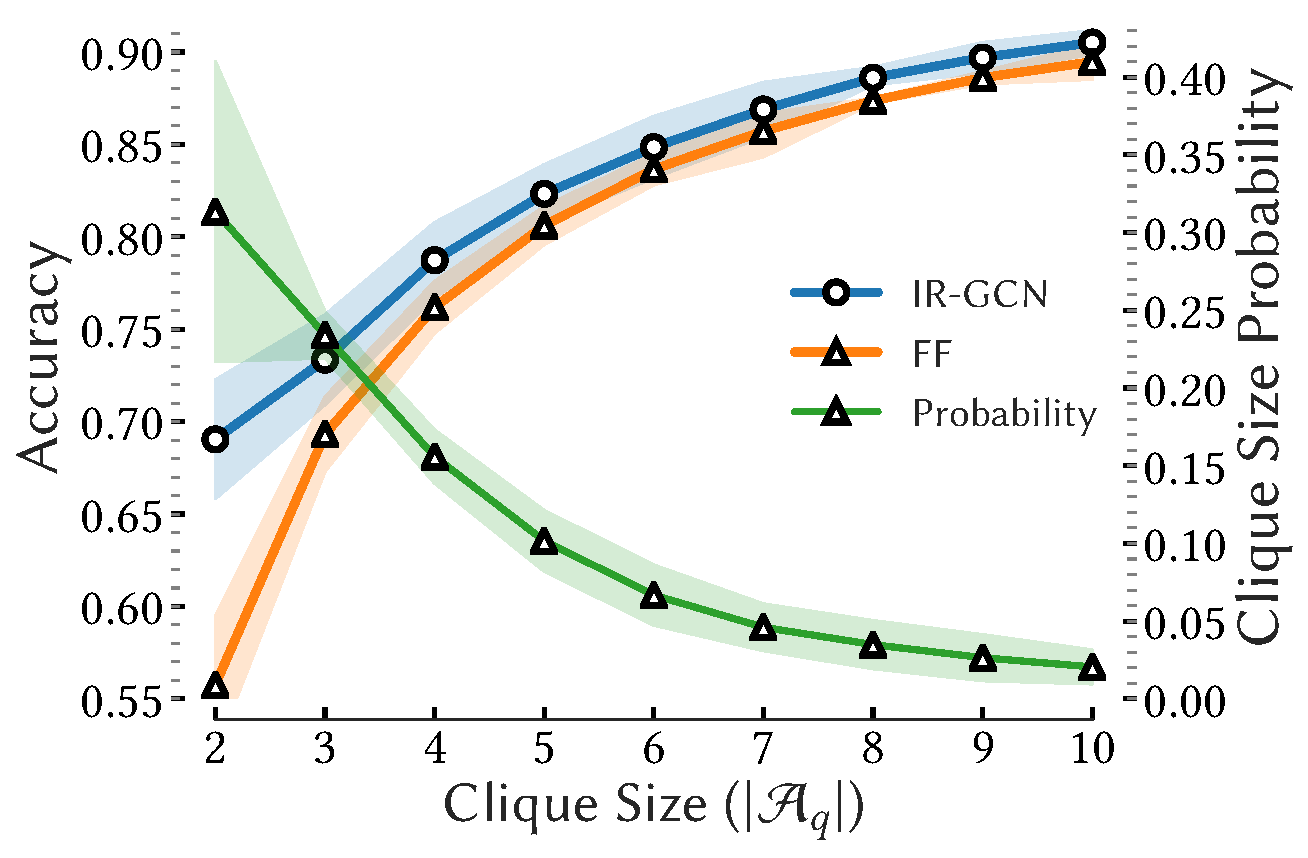
\includegraphics[scale=0.5]{figures/clique_acc.pdf}
  \caption{\label{fig:clique} Accuracy of our IR-GCN model compared to the FF model with varying clique size (i.e. number of answers to a question, $\vert \mathcal{A}_q \vert$) for Contrastive view .
We report averaged results over the largest community of all categories. Our model performs much better for smaller cliques, and the effect diminishes for larger cliques (\cref{eq:contrast}). 80\% of the questions have $< 4$ answers.}
\end{figure}

We show that due to our proposed modification to the convolution operation for contrastive view, we achieve \emph{Discriminative Magnification effect} (\cref{eq:contrast}). Note that the difference is scaled by Clique size ($1 + 1/n-1$), i.e. number of answers to a question, $\vert \mathcal{A}_q \vert$. Figure \ref{fig:clique} shows the accuracy of our IR-GCN model as compared to the FeedForward model with varying clique size. Recall that the FeedForward model predicts node labels independent of other nodes and is not affected by clique size. We report average results over the same five communities as above. We can observe that increase in accuracy is much more for lower clique sizes (13\% improvement for $\vert \mathcal{A}_q \vert = 2$ and 4\% for $\vert \mathcal{A}_q \vert = 3$ on average). The results are almost similar for larger clique sizes. In other words, our model significantly outperforms the FeedForward model for questions with fewer candidate answers. However, around 80\% of the questions have very few answers($< 4$), and thus this gain over FF is significant.

\begin{figure}[h]
      \centering
  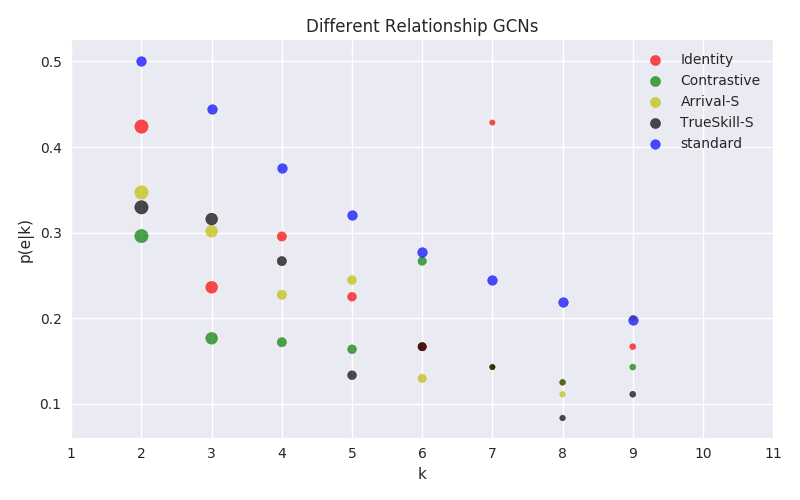
\includegraphics[scale=0.55]{figures/ErrorPlot.png}
  \caption{\label{fig:error} Probability of error with varying clique size for movie StackExchange. Standard represents random selection. Contrastive view outperforms other views for smaller clique sizes.  }
\end{figure}

Alternatively, we also plot the probability of error per tuple given each clique size ($p(e|k)$) for the movie StackExchange in \Cref{fig:error}. The \emph{standard} corresponds to a naive baseline of randomly selecting an accepted answer within each clique. For this standard baseline, error probability per clique can be denoted as,
\begin{align}
p(e|k) = (1 - 1/k) * \frac{2}{k} = \frac{2(k-1)}{k^2}
\end{align}
$(1 - 1/k)$ denotes the probability of choosing the wrong accepted answer, while $2/k$ is the actual error rate in these scenarios. The error rate is such because even in cases where the baseline chose the wrong accepted answer, remaining answers are still correctly classified as not accepted. Thus, there are only two errors per clique.

The standard baseline performs the worst as the error probability is highest than the other baselines for each clique. The Contrastive view has the least error probability for smaller cliques ($k<5$). This result is analogous to the performance gain illustrated above due to the \emph{Discriminative Magnification effect}. For larger cliques, similar contrast views (ArrivalSkill and TrueSkill) have the least error probability. As both of these views connects similar tuples across different questions, they are thus more useful for questions with a higher number of competing answers.



\subsection{Label Sparsity}

\begin{figure}[h]
      \centering
  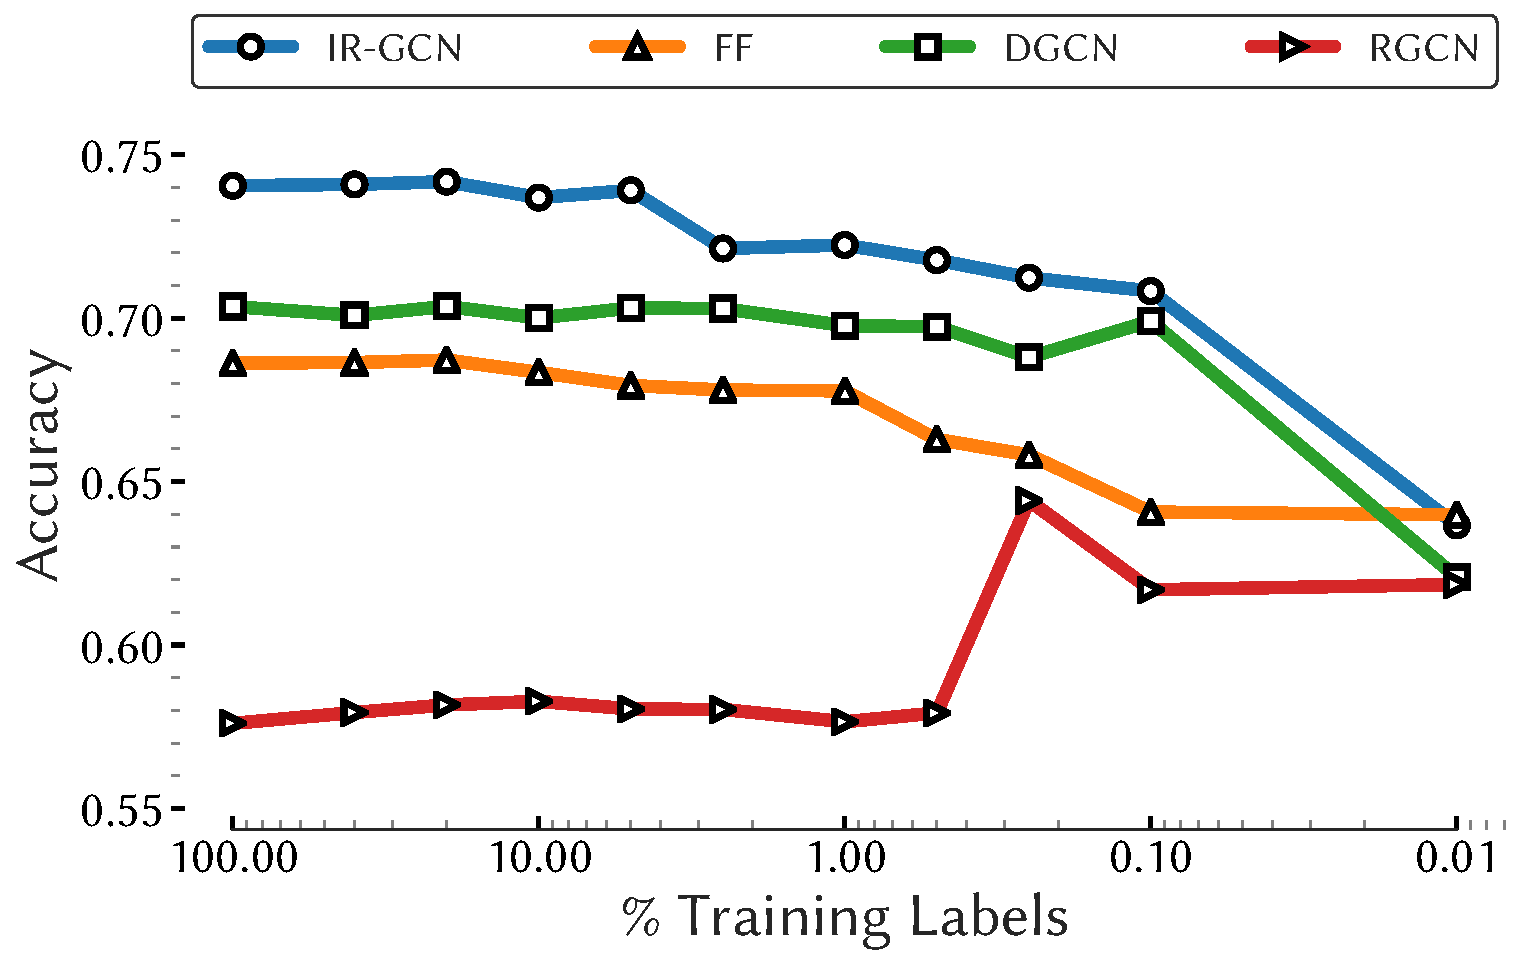
\includegraphics[scale=0.5]{figures/sparsity_acc_physics.pdf}
  \caption{\label{fig:labelsparsity} Change in accuracy with varying training label rates for Physics StackExchange. Our model is more robust to label sparsity than other relation ensemble approaches. RGCN works better with fewer labels as contrastive relation introduces noise in the model. At extreme sparsity, all approaches converge to the same value indicating random selection.}
\end{figure}
Graph Convolution Networks are robust to label sparsity as they exploit graph structure and are thus heavily used for semi-supervised settings. Figure \ref{fig:labelsparsity} shows the change in accuracy for Physics StackExchange from the Science category at different training label rates. Even though our graph contains disconnected cliques, IR-GCN still preserves robustness to label sparsity.
In contrast, the accuracy of the FeedForward model declines sharply with less label information. Performance of DualGCN remains relatively stable while Relational GCN's performance increases with a decrease in label rate. Relational GCN assumes each view to be of similarity relation, and thus, adding contrastive relation introduces noise in the model. However, as the training labels become extremely sparse, the training noise decreases that leads to a marked improvement in the model. In the case of an extremely low label rate of 0.01\%, all approaches converge to the same value, which is the expectation of theoretically random selection. We also obtained similar results for the other four StackExchange communities.


\subsection{Including Textual Features}
Most of the current literature focuses on using textual similarity for Answer Selection. In this section, we compare our proposed IR-GCN model to a popular text-based model~\cite{Tan2015} for answer selection.

\noindent
\textbf{Text Preprocessing}: For this experiment, we first preprocessed the text of both questions and answers.
We first removed all code snippets, HTML tags, stopwords, and URLs from the text of all questions and answers. We then tokenized the text using NLTK tokenizer followed by lemmatization using WordNetLemmatizer and finally converted it into lowercase.

We use torchtext (\url{https://pytorch.org/text/}) to create vocabulary and limit the text of each question and answer to be 250 words long. We initialized the words in the vocabulary using 300-dimensional pre-trained embeddings from Word2vec (\url{https://code.google.com/archive/p/word2vec/}). We randomly initialized words present in the vocabulary but not in word2vec.

We evaluate multiple approaches to test the effectiveness of incorporating textual features for answer selection task.
\noindent
\textbf{QA-LSTM/CNN \cite{Tan2015}} uses a stacked bidirectional LSTM model followed by convolution filters to extract embeddings for the question and answer text separately. Answers are then classified according to the cosine similarity of learned question and answer embedding.

Specifically, in this baseline, we use a biLSTM model with a hidden dimension = 300, followed by 50 1D convolutional filters with a kernel size of 3. We then compute the final embeddings by applying 1D max-pooling on the output of the convolution layer. We also used Tanh nonlinearity and a dropout of 0.3 on the final embeddings. We finally use these embeddings to compute a cosine similarity score between a question and its answers. This score is used to rank the candidate answers for evaluation. We implemented the baseline in Pytorch.

\noindent
\textbf{Textual Similarity (T-GCN)} We create a \textit{SimilarContrast} view that connects answers authored by a user where her answer is significantly similar (dissimilar) to the question than other competing answers. We used cosine similarity on the learned question and answer embedding from the QA-LSTM/CNN approach as the similarity function.

Specifically, we extract the updated embeddings of the question and answer text from the learnt QA-LSTM model. We then compute cosine similarity between the embeddings of each question and its answers.
We then connect answers authored by a specific user, where the difference in cosine similarity of the answer with the other competing answers is greater than margin $\lambda$. Specifically, if the user authors answers $a, a'$ to questions $q, q'$, we create a link between $a$ and $a'$ if
\begin{align}
 \lvert C_{q,a} - C_{q, b} \rvert &> \lambda; \forall b \in \mathcal{A}_(q) \\
 \lvert C_{q,a'} - C_{q, c} \rvert &> \lambda; \forall c \in \mathcal{A}_(q')
\end{align}
where $C_{q,a}$ is the cosine similarity of the answer $a$ with respect to question $q$. Similarly, a link is created for the opposite case when difference is less than $-\lambda$. In our experiments, we assign $\lambda = 0.4$. The hypothesis is that irrelevant(dissimilar) answers will more likely be rejected and vice versa.

\noindent
\textbf{IR-GCN + T-GCN} extends our proposed model to also include the Textual Similarity as the third \textit{SimilarContrast} view in addition to Arrival and TrueSkill Similarity.

\begin{table}[h]
  \centering
  \begin{tabular}{l | S[round-mode=places,round-precision=2]S[round-mode=places,round-precision=2]S[round-mode=places,round-precision=2]S[round-mode=places,round-precision=2]S[round-mode=places,round-precision=2]}
    \toprule
    {Method} &
      {Tech} &
      {Culture} &
      {Life} &
      {Sci} &
      {Business}\\
      \midrule
    QA-LSTM/CNN\cite{Tan2015} & 66.49 & 71.70  & 69.42 & 62.91 & 72.55 \\
    FF~\cite{JendersKN16} & 68.30 & 73.35 & 76.57 & 67.40 & 75.76 \\
    C-GCN & 71.23 & 75.90 & 78.71 & 72.99 & 76.85 \\
    T-GCN & 69.25 & 73.77 & 76.39 & 67.79 & 77.08\\
    IR-GCN & 73.87 & 78.74 & 81.60 & 74.68 & 80.56 \\
    IR-GCN + T-GCN & 73.89 & 78.00  & 81.07 & 74.49 & 78.86\\
    \bottomrule
  \end{tabular}
  \caption{\label{tab:text} 5-fold Accuracy comparison of text-based baseline and textual similarity GCN with IR-GCN.}
\end{table}

In general, the text-based baseline, QA-LSTM, performs worse than even reflexive GCN, as shown in Table \ref{tab:text}. Note that reflexive GCN employs a feedforward model on the activity and user features used in our experiments. This worse performance is surprising as most of the current literature focuses on textual features for the task. Our results indicate that non-textual features are useful too for answer selection task on StackExchange communities.

Textual Similarity GCN performs better than QA-LSTM and Reflexive GCN. Even though we use the output of QA-LSTM to construct the graph for T-GCN, the graph improves performance as it connects answers across questions. However, adding the T-GCN view in our proposed IR-GCN model decreases the performance slightly. One possible explanation could be that similar contrast views based on user features (Arrival similarity and TrueSkill similarity) are not compatible with views based on textual features.

\begin{table}[h]
  \centering
  \begin{tabular}{l | S[round-mode=places,round-precision=2]S[round-mode=places,round-precision=2]S[round-mode=places,round-precision=2]S[round-mode=places,round-precision=2]S[round-mode=places,round-precision=2]}
    \toprule
    {Method} &
      {Tech} &
      {Culture} &
      {Life} &
      {Sci} &
      {Business}\\
      \midrule
    QA-LSTM/CNN\cite{Tan2015} & 66.49 & 71.70 & 69.42 & 62.91 & 72.55 \\
    FF~\cite{JendersKN16} & 66.00 & 72.22 & 69.85 & 63.63 & 75.57 \\
    C-GCN & 66.19 & 72.45 & 70.23 & 63.89 & 75.71 \\
    CT-GCN & 66.06 & 72.35 & 71.88 & 64.14 & 75.69 \\
    IR-GCN & 66.56 & 72.92 & 72.54 & 65.11 & 75.95 \\
    IR-GCN + T-GCN & 66.49 & 73.17 & 72.85 & 65.29 & 75.86 \\
    \bottomrule
  \end{tabular}
  \caption{\label{tab:textfeature} 5-fold Accuracy comparison of text-based baseline and textual similarity GCN with learnt text embeddings as features in the GCN.}
\end{table}

We further replaced our activity-based features with the learned embeddings obtained after training the QA-LSTM/CNN~\cite{Tan2015} model as the node features. We observed that the performance of all approaches went down slightly when using textual features only (Table \ref{tab:textfeature}). As we noted before, GCNs aggregate features among the neighbors. In our similar contrast views, it is not favorable to aggregate textual features among the neighbors as it connects answers catering to different questions. Thus, aggregating textual features creates noise in the model leading to worse performance \footnote{We also experimented with concatenating textual features with the original features used in the previous experiments. However, the performance was still a little worse than the results with only original features.}.


\subsection{Contrastive GCN Analysis}
\label{ref:analysis}
The ability of neural networks to perform classification in sparse high-dimensional manifolds has been studied in past work, especially in the context of adversarial learning \cite{lu2017safetynet}. We employ the ReLU activation function in our convolution layers and study the outputs of the $k$th layer, i.e., embeddings with k-order locality. This transformation breaks the input space into cells with smooth gradients within each cell, at whose boundaries the piecewise linear function changes (i.e., the likelihood of the two classes of answers).

We ask a specific question in the context of our Contrastive GCN. \emph{What is the impact of the layerwise discriminative magnification induced by our formulation?} Discriminative magnifications result in improved separability of the two classes in the later convolving layers, an effect we earlier demonstrated with a sample network in \cref{fig:contrast}. This positively impacts the ability of the model to explain the observed data points (i.e., create p-domains that are well aligned with the contrastive samples provided) and improve the generalizability of the learned model to unseen data points. However, it is crucial to maintain sufficient regularization with weight decay to prevent sparse regions exhibiting sharp gradients that could affect model performance.

The capacity of our model can also be quantified in terms of the VC dimension of the aggregated classifier against the individual learners. Gradient boosting with multiple relation learners (each of which captures a specific aspect of node locality via graph convolution on the induced relations) could boost the capacity of the joint model, enabling better generalization and a more accurate fit in the data manifold (i.e., higher capacity to fit regions to fine distinctions).

Let us denote the upper bound of the VC dimension or capacity of each individual learner as D (If the individual learners do not have identical capacity, the minimum can be used to compute a lower bound on the aggregated learner capacity). Then the gradient boosted learner with T classifiers has a bound on it's capacity~\cite{shalev2014understanding} given by,
\begin{equation}
\mathcal{VC}_{Agg}  = T \times (D+1) \times(3 \log(T.(D+1))+2)
\label{vcdim}
\end{equation}

Thus we identify two potential reasons for our performance gains, first the discriminative magnification effect that also supports the strong individual performance of the contrast view, and second the gain in capacity from boosting, which could explain its advantage over competing aggregation methods.



\subsection{Limitations} We do recognize certain limitations of our work. First, we focus on equivalence relations that induce a graph comprising cliques. While cliques are useful graph objects for answer selection, equivalence relations may be too restrictive for other problems (e.g., the relation is not transitive). However, our modular framework does apply to arbitrary graphs, except that~\Cref{eq:restrictk} will no longer be an \emph{exact} convolution but be an approximation. Second, we assume no evolution in author skills. This assumption is not correct as users evolve with experience. We aim to address this in future work.

In summary, our model showed significant gains over state-of-the-art baselines for combining information from semantically different relational links in a graph. Our model is also more robust to training label sparsity as compared to other aggregator GCN approaches. We reasoned that the performance gains achieved by our aggregation strategy could be attributed in part to the enhanced learning capacity of the boosted model and the effect of discriminative feature magnification. We showed that content can also be used to induce graphs and performs better than using content features in isolation. Finally, we presented a few limitations and possible future extensions.
